% Intended LaTeX compiler: pdflatex
\documentclass[a5paper]{memoir}
\makeatletter

\usepackage{vocabulary}

\def\maketitle{}

\usepackage{eso-pic}

\newcommand*{\casesLegendHeaderBG}{%
  \AddToShipoutPictureBG{%
    \put(\LenToUnit{\paperwidth-25mm-\spinemargin},\LenToUnit{\paperheight-84mm}){%
      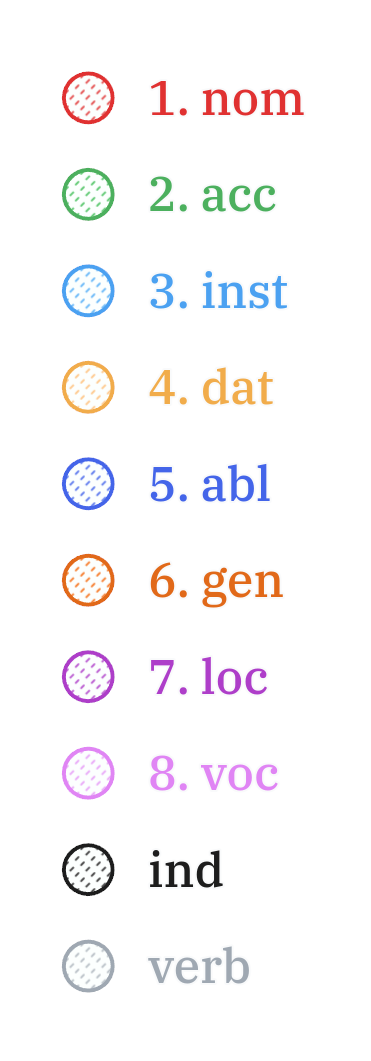
\includegraphics[width=25mm]{./images/cases-legend-white-large.png}%
    }%
  }%
}

\newcommand*{\casesLegendHeaderBGHere}{%
  \AddToShipoutPictureBG*{%
    \put(\LenToUnit{\paperwidth-25mm-\spinemargin},\LenToUnit{\paperheight-84mm}){%
      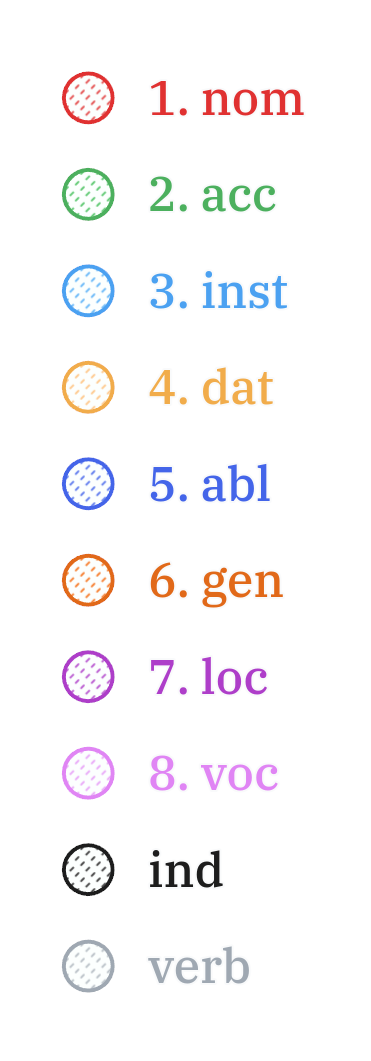
\includegraphics[width=25mm]{./images/cases-legend-white-large.png}%
    }%
  }%
}


\makeatother

\setcounter{secnumdepth}{2}
\date{\today}
\title{Vocabulary: Sentences}
\hypersetup{
 pdfauthor={The Bhikkhu Saṅgha},
 pdftitle={Vocabulary: Sentences},
 pdfkeywords={},
 pdfsubject={},
 pdfcreator={Emacs 29.4 (Org mode 9.6.15)}, 
 pdflang={English}}
\begin{document}


\chapter{Vocabulary: Sentences}
\label{sec:org44d2f13}

\begin{longtable}{L{0.48\linewidth} L{0.48\linewidth} H}
A bhikkhu gives a bowl to a bhikkhu. & bhikkhu bhikkhussa pattaṁ deti & s\\[0pt]
A bhikkhu walks to a village with a bhikkhunī. & bhikkhu bhikkhuniyā gāmaṁ carati & s\\[0pt]
A bone covered with skin; it looks beautiful with clothes. & Aṭṭhi tacena onaddhaṁ, saha vatthebhi sobhati. & s\\[0pt]
A cup of cold water will be refreshing (healthy). & Sītodakamallako kallako bhavissati. & s\\[0pt]
A cup with hot water is a good idea (agreeable thought). & Mallako uṇhodakassa vitakkaṁ piyarūpaṁ. / Uṇhodaka'mallako vitakko piyarūpo (hoti). & s\\[0pt]
After burning the tree with fire, they may make ash. & Rukkhaṁ agginā jhāpetvā masiṁ kareyya. & s\\[0pt]
After eating the food, I rinse my bowl, clean my teeth and go to the hall. & Ahaṁ odanaṁ bhuñjitvā, pattaṁ dhovitvā, dante sodhetvā, sālaṁ gacchāmi. & s\\[0pt]
After sitting down there, he stands up from there. & So tatra nisīditvā tato uṭṭhāti / uṭṭhahati. & s\\[0pt]
After staying here today, tomorrow we go there. & Mayaṁ ajja idha vasitvā suve tahiṁ gacchāma. & s\\[0pt]
After the meal, we should sweep the place. & Pacchābhattaṁ, taṇṭhānaṁ sammajjeyyāma. & s\\[0pt]
All the boys are crying. & Sabbepime dārakā rodanti. & s\\[0pt]
An assembly such as this is worth traveling many leagues to see. & Yathārūpaṁ parisaṁ alaṁ yojanagaṇanānipi dassanāya gantuṁ. & s\\[0pt]
And have you not had trouble getting almsfood? (And not, with the almsfood, you are tired?) & Na ca piṇḍakena kilantosi? & s\\[0pt]
and I'm not tired, friend, from traveling. & \ldots{} appakilamathena cāhaṁ [ca ahaṁ], āvuso, addhānaṁ āgato. & s\\[0pt]
and the other two still attend schools. & dve tāva pāṭha-sālāsu uggaṇhanti. & s\\[0pt]
And where are you now? & Idāni katthañca hosi? & s\\[0pt]
And where do you live Sir? & Katthañca vasatha bhante? & s\\[0pt]
And where from, you Ven., have you come? & Kuto ca tvaṁ bhante, āgacchasi? & s\\[0pt]
Are you able to converse ``into'' Pāli? & Sakkosi tvaṁ pālibhāsāya sallapituṁ? & s\\[0pt]
Are you at your mother and father's house? & Api nu Idāni mātāpitūgāraṁ / -garamhi / -gare viharasi? & s\\[0pt]
Before the meal, we should put out seats. & Purebhattaṁ, āsane / āsanāni paññāpema. & s\\[0pt]
Be heedful! (i.e. take care!) & Appamādosi! & s\\[0pt]
Bhikkhus, I allow bean broth. & ``Anujānāmi, bhikkhave, akaṭayūsan''ti. & s\\[0pt]
Bhikkhus, I allow rice water (clear congee). & ``Anujānāmi, bhikkhave, acchakañjin''ti. & s\\[0pt]
Birds fly in the sky. & Sakuṇā ākāse uḍḍayanti. & s\\[0pt]
But by non-hatred is calmed, this truth is eternal. & Averena ca sammanti, esa dhammo sanantano. & s\\[0pt]
By means of the Teaching, men go to the far shore. & Manussā dhammena pāraṁ gacchanti. & s\\[0pt]
By this truth may there be well-being. & Etena saccena suvatthi hotu. & s\\[0pt]
Come here, layman! & Ehi / Āgacchāhi upāsaka! & s\\[0pt]
Discontent is a dauther of Māra. & Aratī ekā māradhītarā. & s\\[0pt]
Don't go! (imperative) & Mā gaccha! & s\\[0pt]
Do you delight, ascetic? & Nandasi, samaṇa? & s\\[0pt]
Do you go? & Api nu / Kiṁ gacchasi? & s\\[0pt]
Do you have brothers and sisters too? & Tuyhaṁ bhātu-bhaginiyo pi santi? & s\\[0pt]
Do you know Pāli-talk? & Tvaṁ pālibhāsaṁ jānāsi? & s\\[0pt]
Do you like this place? & Piyāyasi tvam idaṁ ṭhānaṁ? & s\\[0pt]
(Due to the) first jhāna there is delight in solitude. & Paṭhamena jhānena suññāgāre abhirati. & s\\[0pt]
Fire, having rose up, burns down the householder's house. & Aggi uṭṭhāya gahapatikassa gehaṁ ḍahati. & s\\[0pt]
for (inspiring) faith in those without faith & appasannānaṁ pasādāya & s\\[0pt]
for restraining obstinate individuals & dummaṅkūnaṁ puggalānaṁ niggahāya & s\\[0pt]
for the ease of the Saṅgha & saṅghaphāsutāya & s\\[0pt]
for the ease of well-behaved monks & pesalānaṁ bhikkhūnaṁ phāsuvihārāya & s\\[0pt]
for the excellence of the Saṅgha & saṅghasuṭṭhutāya & s\\[0pt]
for the growth of faithful individuals & pasannānaṁ bhiyyobhāvāya & s\\[0pt]
For the personal achieving of the escape (and) extinguishing of all suffering & Sabbadukkha nissaraṇa nibbāna sacchikaranatthāya \ldots{} & s\\[0pt]
for the restraint of presently visible (mental) effluents & diṭṭhadhammikānaṁ āsavānaṁ saṁvarāya & s\\[0pt]
for the warding off of future (mental) effluents & samparāyikānaṁ āsavānaṁ paṭighātāya & s\\[0pt]
For what purpose have you come? (You what to do came?) & Tvaṁ kiṁ kātuṁ āgato'si? & s\\[0pt]
From here, to where do you go? & Ito tvaṁ kuhiṁ gacchasi? & s\\[0pt]
Give congee, give rice, give food! & Yāguṁ detha, bhattaṁ detha, khādanīyaṁ dethā! & s\\[0pt]
Go at your convenience. & Yassadāni tumhe kālaṁ maññatha. & s\\[0pt]
Go at your convenience. & Yassadāni tvaṁ kālaṁ maññasi. & s\\[0pt]
Go away, beings! & Paṭikkamantu bhūtāni! & s\\[0pt]
Good morning friend! Are you well? & Suppabhātaṁ āvuso. Kacci si khamanīyaṁ? & s\\[0pt]
Have you not had trouble? (not tired/weary you are '√as') & Na kilantosi? & s\\[0pt]
Having approached, he greeted the Blessed One. & Upasaṅkamitvā bhagavatā saddhiṁ sammodi. & s\\[0pt]
Having been washed, they should be dried. & Dhovitvā, visoseyyāsi / visosetabbāni. & s\\[0pt]
Having come here, having cooked, they go. & Te idha āgantvā pacitvā gacchanti. & s\\[0pt]
Having eaten, having drunk, you lie down. & Tvaṁ buñjitvā pivitvā sayasi. & s\\[0pt]
Having eaten, I don't want to lie down. & Ahaṁ bhuñjitvā sayituṁ na icchāmi. & s\\[0pt]
Having given this robe, may you let me go forth Sir, out of compassion. & \ldots{} etaṁ kāsāvaṁ datvā, pabbājetha maṁ bhante, anukampaṁ upādāya. & s\\[0pt]
Having heard that teaching we know thus\ldots{} & Mayaṁ taṁ dhammaṁ sutvā evaṁ jānāma\ldots{} & s\\[0pt]
Having taken my bowl, the alms should be shared with the bhikkhus. & Me pattaṁ gahetvā / ādāya, piṇḍaṁ bhikkhūhi saddhiṁ saṁvibhajitabbaṁ. & s\\[0pt]
Having walked for alms, having received a lot of food, my bowl is heavy. & Piṇḍāya caritvā / gatvā, bahu khādanīyaṁ paṭiggahetvā / labbhitvā, me patto garo. & s\\[0pt]
Having washed my bowl, you should put (it) in the cupboard. & Me pattaṁ dhovitvā, koṭṭhake odaheyya. & s\\[0pt]
He confesses the offense. & Āpattiṁ āvikaroti. & s\\[0pt]
he doesn't achieve rapture and bliss & pītisukhaṁ nādhigacchati & s\\[0pt]
He, from the breakup of the body, from after death\ldots{} & So, kāyassa bhedā, paraṁ maraṇā \ldots{} & s\\[0pt]
He gives her the cloth. & So tassā dussaṁ deti. & s\\[0pt]
He, having gone there, comes here. & So tatra gantvā idha āgacchati. & s\\[0pt]
He needed bean broth. & Akaṭayūsena attho hoti. & s\\[0pt]
He needed rice water (clear congee). & Acchakañjiyā attho hoti. & s\\[0pt]
Here, bhikkhus, a bhikkhu observes the body in the body\ldots{} & Idha, bhikkhave, bhikkhu kāye kāyānupassī viharati \ldots{} & s\\[0pt]
Here he rejoices, after (death) he rejoice, the merit-doer rejoices on both sides. & Idha modati pecca modati, katapuñño ubhayattha modati. & s\\[0pt]
Here in the morning it is cold, and in the daytime is it hot. & Idha pubbaṇhasamaye ca sīto hoti, majjhanhikasamaye ca uṇho hoti. & s\\[0pt]
Here, the merchant is my friend. & Idha vāṇijo mayhaṁ mitto hoti. & s\\[0pt]
He should sweep the floor and he should expel the ants with this broom. & Chamā ca sammajjeyya, kipillikā ca nikkaḍḍheyya iminā sammuñjaniyā. & s\\[0pt]
He speaks with our given consent and approval. & Chandañca ruciñca ādāya voharati. & s\\[0pt]
He wanders about with a woman. & Mātugāmena saddhiṃ cārikaṁ carati. & s\\[0pt]
He wishes to stay here. & So idha vasituṁ icchati. & s\\[0pt]
Hey layman, come here! & Ehi upāsaka! & s\\[0pt]
Homage to him, the Blessed One. & Namo tassa bhagavato. & s\\[0pt]
Homage to the Buddha. & Namo Buddhāya / Buddhassa. & s\\[0pt]
How are you untroubled, mendicant? How is delight not found in you? & Kathaṁ tvaṁ anagho bhikkhu, kathaṁ nandī na vijjati? & s\\[0pt]
How, as you sit alone, does discontent not overwhelm you? & Kathaṁ taṁ ekamāsīnaṁ, aratī nābhikīrati? & s\\[0pt]
How can I help (do)? & Kinti karomi? & s\\[0pt]
How can I help (do), Sir? & Kinti karomi bhante? & s\\[0pt]
How much (many) money have you now with you? & Kittakaṁ mūlaṁ 'dāni tava santike atthi? & s\\[0pt]
How old are you? (How many years are you?) & Kativasso'si tvaṁ (āyunā)? & s\\[0pt]
I am alright. & Ahaṁ khamanīyo / Khamanīyaṁ me. & s\\[0pt]
I am a way-farer. & Aham eko pathiko. & s\\[0pt]
I am called Vijayabāhu. & Ahaṁ Vijayabāhu-nāmo'mhi. & s\\[0pt]
I am entering the town Ericeira. & Ericeiraṁ pavisāmi. & s\\[0pt]
I am not well. & Na me, bhante, khamanīyaṁ. & s\\[0pt]
I am not well, Sir. I feel cold. & Na me, bhante, khamanīyaṁ. Sītaṁ vedayāmi / paṭisaṁvediyāmi. & s\\[0pt]
I am tired. (Me tired I am '√as') & Ahaṁ kilantosmi. [kilanto + asmi] & s\\[0pt]
I am twenty years old. & Ahaṁ vīsativasso'mhi. & s\\[0pt]
I came here to talk to you. (Wit you to talk came I am.) & Tayā saddhiṁ sallapituṁ āgato'mhi. & s\\[0pt]
I come from India. & Ahaṁ Indudesato āgacchāmi. & s\\[0pt]
I don't know. Do you see it? & Na jānāmi. Taṁ passasi? & s\\[0pt]
I enter the empty hut. & Suññāgāraṁ pavisāmi. & s\\[0pt]
If, after stealing, he might come here, I may punish (him). & Sace so coretvā idha āgacceyya, daṇḍaṁ paṇeyyāmi. & s\\[0pt]
If he might not produce it\ldots{} & No ce abhinipphādeyya\ldots{} & s\\[0pt]
If he should keep it longer than that\ldots{} & Tato ce uttariṁ nikkhipeyya\ldots{} & s\\[0pt]
If only we could not be of the nature to die! & Aho vata mayaṁ na maraṇadhammā assāma! & s\\[0pt]
If the assembly hall is dirty, it should be swept. & Sace upaṭṭhānasālā uklāpā hoti, upaṭṭhānasālā sammajjitabbā. & s\\[0pt]
If there's no drinking water, drinking water should be provided. & Sace pānīyaṁ na hoti, pānīyaṁ upaṭṭhāpetabbaṁ. & s\\[0pt]
If there's no rinsing water, rinsing water should be provided. & Sace paribhojanīyaṁ na hoti, paribhojanīyaṁ upaṭṭhāpetabbaṁ. & s\\[0pt]
If the teacher wants coffee, we should prepare coffee. & Sace ācariyaṁ kāphīpānaṁ icchati, kāphīpānaṁ paṭiyādema. & s\\[0pt]
If you want water, please tell me Sir. & Sace udakaṁ icchasi, vadetha me bhante. & s\\[0pt]
I got more food than (of) Ven. Kovilo. I will share with him. & Āyasmato Kovilassa bahutaraṁ āhāraṁ labbhāmi. Ahaṁ tena vibhajissāmi. & s\\[0pt]
I had no trouble getting almsfood. (tired I am '√as') & Na ca piṇḍakena kilantomhi. & s\\[0pt]
I have fourteen rupees. & Cuddasa rūpiyāni mama santike santi. & s\\[0pt]
I hope you all are well. & Kacci vo khamanīyaṁ. & s\\[0pt]
I hope you are well (enduring)? & Kacci te bhante khamanīyaṁ? & s\\[0pt]
I hope you are with little fatigue? & Kacci'si appakilamathena? & s\\[0pt]
I hope you're keeping well Ven., I hope you're getting by? & Kacci, bhante, khamanīyaṁ kacci yāpanīyaṁ? & s\\[0pt]
I hope you're with little fatigue from traveling? & Kacci'si appakilamathena addhānaṁ āgato? & s\\[0pt]
I know a little. & Ahaṁ thokaṁ jānāmi. & s\\[0pt]
I like to become an architect. (I an architect to become desire.) & Aham eko gahakāraṁ bhavitum icchāmi. & s\\[0pt]
I live in Colombo-town. & Ahaṁ Koḷambanagare vasāmi. & s\\[0pt]
I live in Norway. There it is always cold. & Norway janapade vasāmi. Tatra sītaṁ sabbadā. & s\\[0pt]
I may like this place, if it doesn't get too hot. (if here not too hot may become). & Piyāyeyyam idaṁ ṭhānaṁ sace'daṁ nāccuṇhaṁ bhaveyya. & s\\[0pt]
I'm keeping well, friend, I'm getting by. & Khamanīyaṁ, āvuso, yāpanīyaṁ. & s\\[0pt]
I must go now. Bye for a week. & Handa dāni ahaṁ gacchāmi. (Anantaraṁ) sattāhaṁ. & s\\[0pt]
Indeed not by hatred, that hatred is calmed, at any time. & Na hi verena verāni, sammant'īdha kudācanaṁ. & s\\[0pt]
In the region (of) \ldots{}, is it hot? & Api nu \ldots{}-dese uṇho hoti? & s\\[0pt]
In the town called Ericeira, there is the market. I go there for alms. & Gāme Ericeira nāmo, atthi antarāpaṇo. Tatra piṇḍāya gacchāmi. & s\\[0pt]
I plow and sow. & Ahaṁ kasāmi vapāmi ca. & s\\[0pt]
I see the moon. & Candaṁ passāmi. & s\\[0pt]
It leads to Nibbāna. & Nibbānāya saṁvattati. & s\\[0pt]
I, together with a friend, go to the village. & Ahaṃ mittena saddhiṃ gāmaṁ gacchāmi. & s\\[0pt]
I trust Sir (you) slept well? & Kacci bhante sukhamasayittha? & s\\[0pt]
I use the requisite. & Parikkhāraṁ paṭisevāmi. & s\\[0pt]
I want to sell some goods. & Ahaṁ bhaṇḍāni vikkiṇitum icchāmi. & s\\[0pt]
I (we) must go. & Handa dāni mayaṁ gacchāma. & s\\[0pt]
I will go to another town from here. (I from here to another town I will go.) & Aham ito aññaṁ nagaraṁ / nigamaṁ gamissāmi. & s\\[0pt]
I will go to the forest to see the Buddha. & Ahaṁ buddhaṁ passituṁ araññaṁ gacchissāmi. & s\\[0pt]
I will wash your cup. & Tuyhaṁ mallakaṁ dhovāmi / dhovissati. & s\\[0pt]
I work in a post-office. (I in one marketplace work I do.) & Aham ekasmiṁ antarāpaṇe kammaṁ karomi. & s\\[0pt]
Let him live comfortably! & Phāsu viharatu! & s\\[0pt]
Let the Sangha hear me. & Suṇātu me bhante saṅgho \ldots{} & s\\[0pt]
Let the Venerables declare purity. & Pārisuddhiṁ āyasmanto ārocetha. & s\\[0pt]
Like rivers full of water\ldots{} & Yathā vārivahā pūrā\ldots{} & s\\[0pt]
May all beings be happy. & Sabbe sattā sukhī hontu. & s\\[0pt]
May all misfortunes be avoided, may all illness be dispelled. & Sabbītiyo vivajjantu sabbarogo vinassatu. & s\\[0pt]
May either he or she go. & So vā sā vā gacchatu. & s\\[0pt]
May he come here. (imperative) & Idha āgacchatu. & s\\[0pt]
May the Buddha accept (that) transgression. & Buddho paṭiggaṇhātu accayantaṃ. & s\\[0pt]
May the master come here. (imperative) & Ayyo idha āgacchatu. & s\\[0pt]
May they burn the defilements! & Kilese tapantu! & s\\[0pt]
May they delight in meditation, may they go to the devas. & Bhāvanābhiratā hontu, gacchantu devatā-gatā. & s\\[0pt]
May they give gifts with conviction, may they always maintain virtue. & Dānaṃ dadantu saddhāya, sīlaṃ rakkhantu sabbadā. & s\\[0pt]
May you feel calm! & Samitaṁ vedehi! & s\\[0pt]
May you live 100 years! & Vassasataṁ jīva! & s\\[0pt]
May you not burn with sensual desire! & Kāmarāgena mā ḍayhatha! & s\\[0pt]
(May you) Sleep well! & Sukhaṁ sehi! & s\\[0pt]
Monkeys move about on trees. & Makkaṭā rukkhesu vicaranti. & s\\[0pt]
My age is fifteen. & Mayhaṁ āyuppamāṇaṁ paṇṇarasa. & s\\[0pt]
My father is the merchant Mahānāma. & Mama pitā Mahānāmo vāṇijo. & s\\[0pt]
My name is \ldots{} & Ahaṁ bhante \ldots{} nāma. & s\\[0pt]
My preceptor's name is Ven. \ldots{} & Upajjhāyo me bhante āyasmā \ldots{} nāma. & s\\[0pt]
No friend, I haven't slept well. & No hetaṁ, āvuso, na sukhamasayitthaṁ. & s\\[0pt]
No Sir. I come from the country \ldots{} & No hetaṁ, bhante. \ldots{} janapadasmā āgacchāmi. & s\\[0pt]
not this I am & n'eso'ham'asmi [na + eso + ahaṁ + asmi] & s\\[0pt]
Now rain falls, (so) don't go out. & Idāni devo vassati, mā bahi gacchittha. & s\\[0pt]
Now, we eat here and go there to sow. & Mayaṁ idāni atra bhutvā vapituṁ tahiṁ gacchāma. & s\\[0pt]
Old age falls. & Vayo nipatati. & s\\[0pt]
One of them is a merchant, the second one is a clerk, & Tesu eko vāṇijo, ditiyo lekhako, & s\\[0pt]
on the holy life a defect, crack, stain, blemish & brahmacariyassa khaṇḍampi chiddampi sabalampi kammāsampi & s\\[0pt]
Our bodily behaviour should be purified. & Parisuddho no kāyasamācāro bhavissati. & s\\[0pt]
(Please) Give me (a) toothbrush. & Dantaponaṁ me dehi. & s\\[0pt]
Please sit here. Where does the master go for alms? & Ettheva / Idha nisīdatha. Kuhiṁ / Kathaṁ piṇḍāya ayyo gacchatha? & s\\[0pt]
(Please) Wash my bowl. & Me pattaṁ dhova / dhovatha. & s\\[0pt]
(Please) you could wash these robes (clothes). & Imāni vatthāni dhoveyyāsi. & s\\[0pt]
Prince Abhaya goes up to the Buddha. & Abhayo rājakumāro yena bhagavā ten'upasaṅkamati. & s\\[0pt]
Privately, he takes a seat. & Raho nisajjaṁ kappeti. & s\\[0pt]
Rice cooked by the cook was eaten by the beggar's dog. & Sūdena pacito odano yācakassa sunakhena khādito. & s\\[0pt]
Right here friend. Do you come from the country Spain? & Etthevaṁ āvuso. Spain-desamhā āgacchasi? & s\\[0pt]
She comes from there. & Sā tato āgacchati. & s\\[0pt]
Sitting here, don't cry, go there, having gone and eaten, lie down. & Idha nisīditvā mā rodāhi, tatra gacchāhi, gantvā bhutvā sayāhi. & s\\[0pt]
Taken away by thieves, the householder's oxen are slaughtered. & Corehi haritvā, gahapatino gāvo haññanti. & s\\[0pt]
Thank you friend, I am tired from coming on the journey. & Anumodāmi āvuso. Kilamathena addhānaṁ āgato. & s\\[0pt]
That's where I, Ven., am coming from. & Tato ahaṁ, bhante, āgacchāmi. & s\\[0pt]
The 4 foundations of mindfulness fulfil the 7 factors of enlightenment. & Cattāro satipaṭṭhānā satta bojjhaṅge paripūrenti. & s\\[0pt]
The birds eat the seeds. & Sakuṇā bījāni bhuñjanti. & s\\[0pt]
The birds fly to the sal trees. & Sakuṇā sālarukkhe uḍḍayanti. & s\\[0pt]
The born die. & Jātā mīyanti. & s\\[0pt]
The boys are running. & Dārakā dhāvanti. & s\\[0pt]
The boys eat the food. & Dārakā bhojanīyaṁ bhuñjanti. & s\\[0pt]
The boy stands. & Dārako tiṭṭhati. & s\\[0pt]
The Buddha was wandering in the land of the Kosalans\ldots{} & Bhagavā kosalesu cārikaṁ carati\ldots{} & s\\[0pt]
The chef cooks the rice. & Sūdo bhattaṁ pacati. & s\\[0pt]
The community gives this Kaṭhina-cloth to Ven. Amaro. & Saṅgho imaṃ kaṭhinadussaṃ āyasmato Amarassa deti. & s\\[0pt]
The cooks cook the rice for the householder's servants. & Sūdā gahapatino sevakānaṁ odanaṁ pacanti. & s\\[0pt]
The cup breaks. & Mallako bhindati. & s\\[0pt]
The darkness was dispelled by the sun's light. & Suriyassa ālokena andhakāro apagato. & s\\[0pt]
The disciple eats the lion. & Sāvako sīhaṁ khādati. & s\\[0pt]
The dogs are barking at the cats. & Sunakhā biḷāre bhussanti. & s\\[0pt]
The dogs are barking at the moon. & Sunakhā candaṁ bhussanti. & s\\[0pt]
The elder gives the robe to the disciple. & Thero sāvakassa cīvaraṁ deti. & s\\[0pt]
The elder goes to the village by air. & Thero ākāsena gāmaṁ gacchati. & s\\[0pt]
The elder goes to the village with the disciple (\emph{sāvaka}). & Thero sāvakena saddhiṁ gāmaṁ gacchati. & s\\[0pt]
The elder is going on a walk. & Thero cārikaṁ carati. & s\\[0pt]
The elders make an effort. & Therā viriyaṁ ārabhanti. & s\\[0pt]
The layman doesn't go to the village. & Upāsako gāmaṁ na gacchati. & s\\[0pt]
The lion doesn't see the dogs. & Sīho sunakhe na passati. & s\\[0pt]
The lion eats the disciple. & Sīho sāvakaṁ khādati. & s\\[0pt]
The lions are not running. & Sīhā na dhāvanti. & s\\[0pt]
The lion walks in the village. & Sīho gāme / gāmamhi / gāmasmiṁ carati. & s\\[0pt]
The māluva-seed falls at the base of sal trees. & Māluvābījaṁ sālamūle nipatati. & s\\[0pt]
The man eats rice. & Naro bhattaṁ bhuñjati. & s\\[0pt]
The man sits. & Naro nisīdati. & s\\[0pt]
The man's oxen are slaughtered. & Purisassa goṇo / gāvo haññanti. & s\\[0pt]
The men are cooking. & Narā pacanti. & s\\[0pt]
The men run to the barn. & Narā koṭṭhāgāraṁ dhāvanti. & s\\[0pt]
then, Kālāmas, you should undertake them and abide in them\ldots{} & atha tumhe, kālāmā, upasampajja vihareyyātha. & s\\[0pt]
There are in my bed a lot of ants. & Atthi me sayane bahu kipillikā. & s\\[0pt]
There is no equal to the Tathāgata. & Na samo (equal to) atthi tathāgatena. & s\\[0pt]
There is, Ven., in the country (of) America, the monastery called Clear Mountain. & Atthi, bhante, America janapade Pasannagiri-nāma vihāro. & s\\[0pt]
There is, Ven., in the region (of) Portugal, the monastery called Sumedhārāma. & Atthi, bhante, Portugal-dese Sumedhārāma-nāma vihāro. & s\\[0pt]
The Sangha performs the uposatha. & Saṅgho uposathaṁ karoti. & s\\[0pt]
These things are wholesome \ldots{} lead to long-term happiness, & Ime dhammā kusalā \ldots{} hitāya sukhāya saṁvattanti & s\\[0pt]
these volitions would not lead to affliction & na'y'idaṁ saṅkhārā ābādhāya saṁvatteyyuṁ & s\\[0pt]
The sort of stealing for which kings, having caught a thief, would beat or \ldots{} & Yathārupe adinnādāne rājāno coraṁ gahetvā, haneyyuṁ vā\ldots{} & s\\[0pt]
The wise men are delighted in the Buddha. & Viññuno Buddhe pasannā. & s\\[0pt]
The woman stands up. & Mātugāmo uṭṭhahati. & s\\[0pt]
They fill up the ocean. & Paripūrenti sāgaraṁ. & s\\[0pt]
They give ear. & Te sotaṁ odahanti. & s\\[0pt]
They go forth in the bhikkhu-saṅgha. & Te bhikkhu-saṅghe pabbajanti. & s\\[0pt]
They, having seen the disadvantage in sensual pleasures, \ldots{} & Te kāmesu ādīnavaṁ disvā, \ldots{} & s\\[0pt]
They too now, just live in Colombo. & Te p'idāni Koḷambanagare yeva vasanti. & s\\[0pt]
This is his spoon. Give it to his attendant. & Ayamassa kaṭacchu. Assaṁ / tassaṁ upaṭṭhākaṁ dehi. & s\\[0pt]
This morning I am entering the town Ericeira for alms-round. & Idha pubbaṇhasamayaṁ Ericeira-nigamaṁ piṇḍāya pavisāmi. & s\\[0pt]
Today many men assemble in the village. & Ajja bahū manussā gāme sannipatanti. & s\\[0pt]
together with the Buddha & Buddhena saddhiṁ & s\\[0pt]
together with the teacher & ācariyena / ācariyā saddhiṁ & s\\[0pt]
together with the wise men & viññūhi saddhiṁ & s\\[0pt]
Tomorrow will be hot. Do you want a hot drink? & Suve uṇhaṁ bhavissati. Pānaṁ uṇhaṁ icchasi? & s\\[0pt]
two conditions for the arising of right view & dve paccayā sammādiṭṭhiyā uppādāya & s\\[0pt]
Venerable, may the master come and sit here. & Bhante, ayyo āgacchatu, idha nisīdatu. & s\\[0pt]
Wait right here Sir, I will bring (it to you). & Ettheva bhante, tiṭṭha / tiṭṭhatha. (Taṁ taṁ) āharissāmi. & s\\[0pt]
We are obstructed by birth and death. & Mayaṁ otiṇṇā amha jātijarāmaraṇena. & s\\[0pt]
We don't go there to buy. & Mayaṁ ketuṁ tahiṁ na gacchāma. & s\\[0pt]
We don't like to kill. & Mayaṁ hantuṁ na icchāma. & s\\[0pt]
We don't see the change of the body of the man. & Na passāma manussassa kāyassa vipariṇāmaṁ. & s\\[0pt]
We eat the almsfood not for fun or indulgence\ldots{} & Mayaṁ piṇḍapātaṁ bhuñjāma neva davāya, na madāya\ldots{} & s\\[0pt]
We enter the hut. & Agāraṁ pavisāma. & s\\[0pt]
We go to the roots of trees. & Rukkhamūle gacchāma. & s\\[0pt]
We go up to the layman. & Upāsakaṁ upasaṅkamāma. & s\\[0pt]
Welcome, Sir! May the master come here. I hope you are not tired? & Svāgataṁ bhante. Ayyo idha āgacchatu. Kacci'si appakilamathena? & s\\[0pt]
Well indeed, Sir., I shall be restrained. & Sādhu suṭṭhu bhante saṃvarissāmi. & s\\[0pt]
Well then, ascetic, do you sorrow? & Tena hi, samaṇa, socasi? & s\\[0pt]
We run to the boys. & Mayaṁ dārake dhāvāma. & s\\[0pt]
What can I do for you, Sir? & Kiṁ tuyhaṁ karomi, bhante? & s\\[0pt]
What do you like to be / do? (You what work to do desire?) & Tvaṁ kiṁ kammaṁ kātuṁ icchasi? & s\\[0pt]
What do you think? & Taṁ kiṁ maññasi? & s\\[0pt]
Whatever monk who, arranging with a bhikkhuni\ldots{} & Yo pana bhikkhu bhikkhuniyā saddhiṁ saṁvidhāya\ldots{} & s\\[0pt]
What have I gained, friend? & Kiṁ laddhā, āvuso? & s\\[0pt]
What have I lost, friend? & Kiṁ jīyittha, āvuso? & s\\[0pt]
What is your age? (How many is you life-span?) & Tuyhaṁ āyuppamāṇāṁ kittakaṁ? & s\\[0pt]
What is your name? & Kiṁ nāmo si? & s\\[0pt]
What is your name? & Kinnāmosi? & s\\[0pt]
What is your name? & Tuyhaṁ nāmaṁ kiṁ? Kin nāmo'si? & s\\[0pt]
What is your preceptor's name? & Ko nāma te upajjhāyo? & s\\[0pt]
When did you come here? & Kadā tvaṁ idh'āgato'si? & s\\[0pt]
When (if) you, Bhaddiya, know this by yourself\ldots{} & Yadā tumhe, bhaddiya, attanāva jāneyyātha\ldots{} & s\\[0pt]
When I get money, then I will go home. & Yadā mūlaṁ labhissāmi, tadā'haṁ gamissāmi. & s\\[0pt]
When will you go home? & Kadā tvaṁ nivesanaṁ gacchissasi / gamissasi? & s\\[0pt]
Where do you come from? & Kuto tvam āgacchasi? & s\\[0pt]
Where do you live? & Tvaṁ kattha vasasi? & s\\[0pt]
Where do your parents live? (Your mother-and-father lives where?) & Tuyhaṁ mātāpitaro kuhiṁ vasanti? & s\\[0pt]
Where do you work? (Where the work you do?) & Kattha tvaṁ kammaṁ karosi? & s\\[0pt]
Where is Ven. Vajiro bhikkhu's spoon? & Kattha āyasmato Vajiro bhikkhussa kaṭacchu hoti? & s\\[0pt]
Where is your bowl? & Kattha tuyhaṁ pattaṁ? & s\\[0pt]
Who are you? & Ko'si tvaṁ? & s\\[0pt]
Who here is your friend? & Ko idha tava mitto? & s\\[0pt]
Who is your father? & Ko tuyhaṁ pitā? & s\\[0pt]
Who seeks privacy, he wants solitude. & Yo rahāyati, so vivekaṁ icchati. & s\\[0pt]
Why did you come here? (Why here came are you?) & Kasmā idh'āgato si? & s\\[0pt]
Why is that? Today is not hot. & Taṁ kissa hetu? Na ajj'āccuṇhaṃ / ajjūṇho. & s\\[0pt]
Yes, I am able to converse a little. & Āma, ahaṁ thokaṁ sallapituṁ sakkomi. & s\\[0pt]
Yes, I have four brothers and two sisters. & Āma, mayhaṁ cattāro bhātaro dve bhaginiyo ca santi. & s\\[0pt]
Yes, I know you like to walk. & Āma, ahaṁ jānāmi, tvaṁ carituṁ icchasi. & s\\[0pt]
Yesterday I came here. & Hīyo'ham idh'āgacchiṁ. & s\\[0pt]
You are sitting here. & Idha nisīdasi. & s\\[0pt]
You not make a house again\ldots{} & Puna gehaṁ na kāhasi\ldots{} & s\\[0pt]
You (pl.) don't see the dogs. & Sunakhe na passatha. & s\\[0pt]
Your brothers, what do they do? & Tava bhātaro kiṁ karonti? & s\\[0pt]
\end{longtable}
\end{document}
